%%%%%%%%%%%%%%%%%%%%%%%%%%%%%%%%%%%%%%%%%%%%%%%%%%%%%%%%%%%%%%%%%%%%%%%%%%%%%%%%

\documentclass[12pt, a4paper, oneside]{book}

\input{/home/giatro/.config/user/giatro_packages.tex}

\input{/home/giatro/.config/user/giatro_macros.tex}

\title{Deep Learning\\\small{by DeepLearning.AI}}
\date{\today}
\author{Lucas Paiolla Forastiere}

%%%%%%%%%%%%%%%%%%%%%%%%%%%%%%%%%%%%%%%%%%%%%%%%%%%%%%%%%%%%%%%%%%%%%%%%%%%%%%%%
%%%%%%%%%%%%%%%%%%%%%%%%%%%%%%%%%%%%%%%%%%%%%%%%%%%%%%%%%%%%%%%%%%%%%%%%%%%%%%%%

\begin{document}

\maketitle
\tableofcontents
\newpage

%%%%%%%%%%%%%%%%%%%%%%%%%%%%%%%%%%%%%%%%%%%%%%%%%%%%%%%%%%%%%%%%%%%%%%%%%%%%%

\chapter{Introduction}%
\label{cha:introduction}

The term deep learning refers to training \textit{neural networks}, sometimes
very big neural networks. But what are neural networks?

So let's suppose we want to predict housing prices based on the size of the
house. And let's say we'll use Logistic Regression to do that. But as we know,
house prices can't be negative, so we simply say the value of the house is $0$
if the Logistic Regression would predict something negative.

That's indeed the simplest neural network we can have, we have a single input
\texttt{size} and a single output \texttt{price} and in the middle we have a
single neuron: the logistic regression.

\begin{figure}[h]
\centering
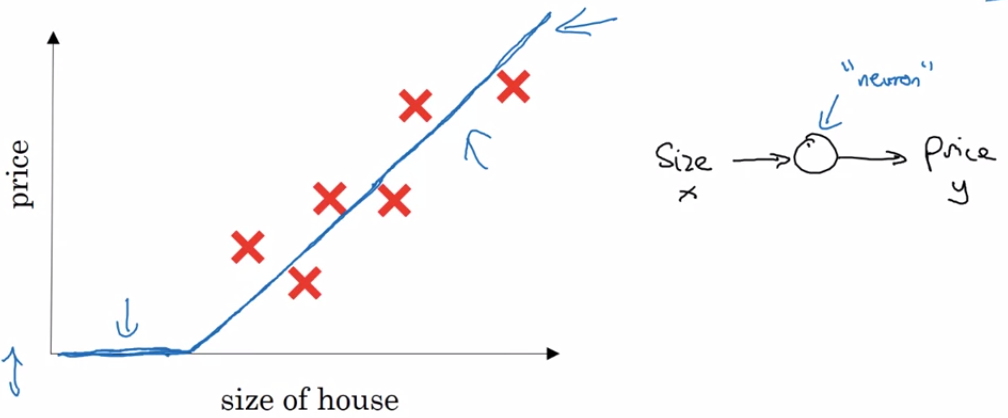
\includegraphics[scale=0.6]{Res/housing_logistic_regression.png}
\caption{Here we see the graph of the problem we described.}
\label{housing_logistic_regression.png}
\end{figure}

That function which is zero and than linear is called \textit{ReLU} and it's
used a lot in neural networks. It stands for \textit{Rectified Linear Unit}.

So to get a bigger neural network, we stack these neurons. Instead of predicting
using only the size of house, we could use the number of bedrooms, zip code and
wealth. We could use the size and number of bedrooms to predict the family size;
use the zip code to predict the walkability; and use the zip code and wealth to
predict the school quality. And then, we could use the family size, walkability
and school quality to predict the price. See in the picture:

\begin{figure}[h]
\centering
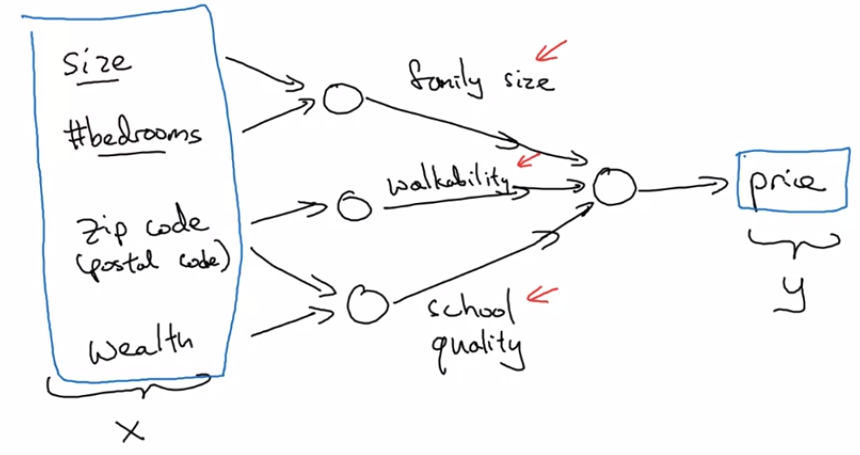
\includegraphics[scale=0.6]{Res/housing_nn.png}
\caption{Now we have a more complex neural network, which is the stack of many
ReLUs.}
\label{/housing_nn.png}
\end{figure}

However, in general what we have is something a little more complex than that.
We would have something like figure \ref{nn_generic.png}. Here we see that the
internal nodes (which are called \textbf{hidden nodes} or \textbf{hidden
neurons} or \textbf{hidden units}) receive the output of all the previous nodes
to make it predictions. These hidden nodes don't really have a meaning like the
example we gave. We don't try to predict family size or walkability or whatever,
we simply let the neural network decide what that neuron will output in order to
predict the final output \texttt{price} in the better way it can.

\begin{figure}[h]
\centering
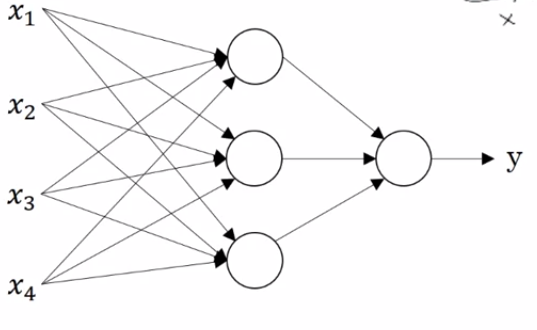
\includegraphics[scale=0.8]{Res/nn_generic.png}
\caption{The generic form of a neural network.}
\label{nn_generic.png}
\end{figure}

We can use neural networks in many applications, here we're going to foucos in
\textbf{supervised learning}, which are problems that you have a set of
variables called input (represented by $x$) and an output ($y$) related to that
input. In order to solve these kind of problems, there are many kinds of neural
networks. The one we saw is the most common one, but there are others, like
convolutional nn or recurrent nn.

\begin{figure}[h]
\centering
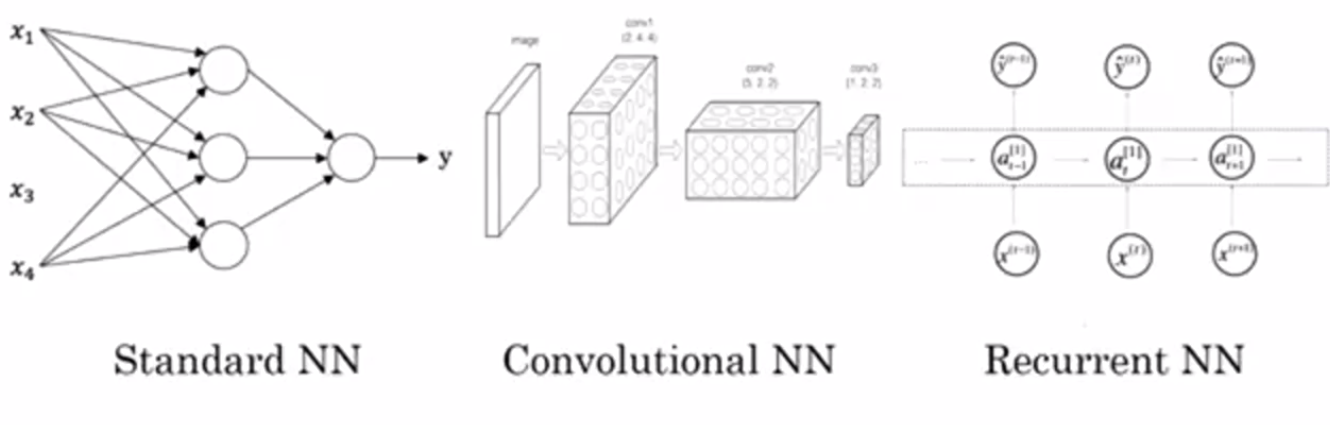
\includegraphics[scale=0.3]{Res/examples_nn.png}
\caption{Examples of neural networks.}
\label{examples_nn.png}
\end{figure}

Another thing that's important to decide what kind of nn we'll use is knowing if
the data we're leading with is \textit{structured} or \textit{unstructured}.

\textbf{Structured data} is data in the form of a table. We have a very clear
set of input variable $X$ and a set of output variables $y$. Each line of our
table represents one instance of data with many inputs and one or more outputs
related to those inputs.

\textbf{Unstructured data} is all the other kinds of data: audio, video, texts,
images, etc.

\begin{figure}[h]
\centering
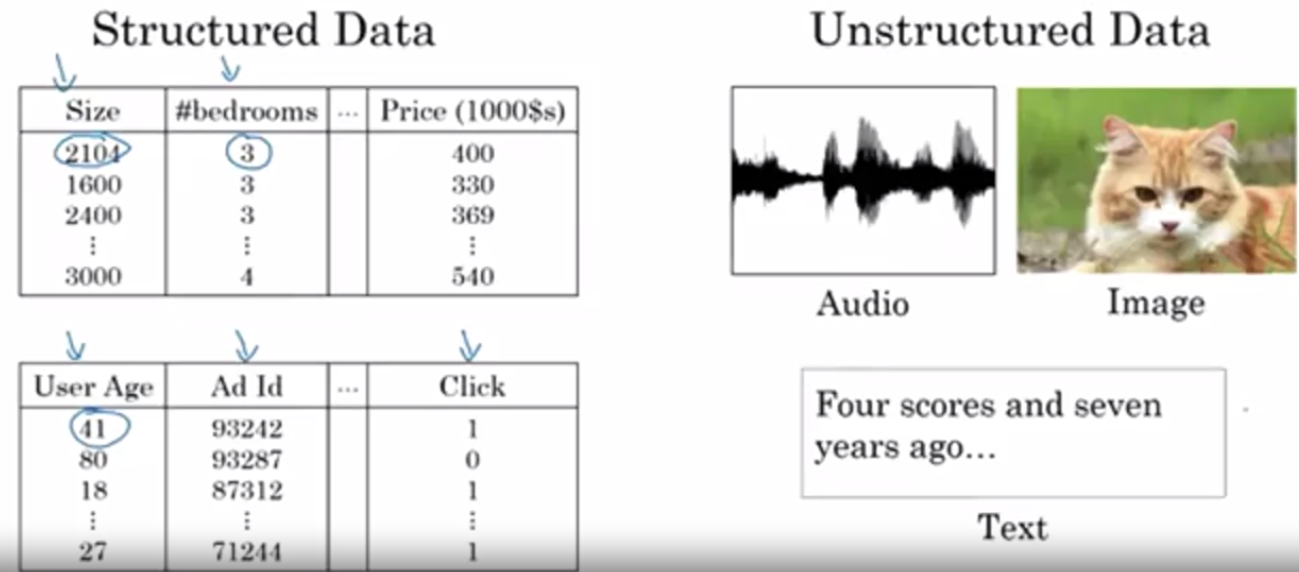
\includegraphics[scale=0.4]{Res/structured_vs_unstructed_data.png}
\caption{The two kinds of data.}
\label{structured_vs_unstructed_data.png}
\end{figure}

It turns out that machine learning algorithms performed better on structured
data over the years and more recently neural networks are performing better also
on unstructured data.

\paragraph{Why is Deep Learning taking off?}%
\label{par:why_is_deep_learning_taking_off_}

This is one of the questions we must ask ourselves when begining to learn deep
learning. Let's see the graph of the performance of the machine learning
algorithms versus the amount of data that we provide to then. We see that
traditional learning algorithms have a plato where they can't improve anymore,
which neural networks can lead with that data as we make than bigger and bigger.

\begin{figure}[h]
\centering
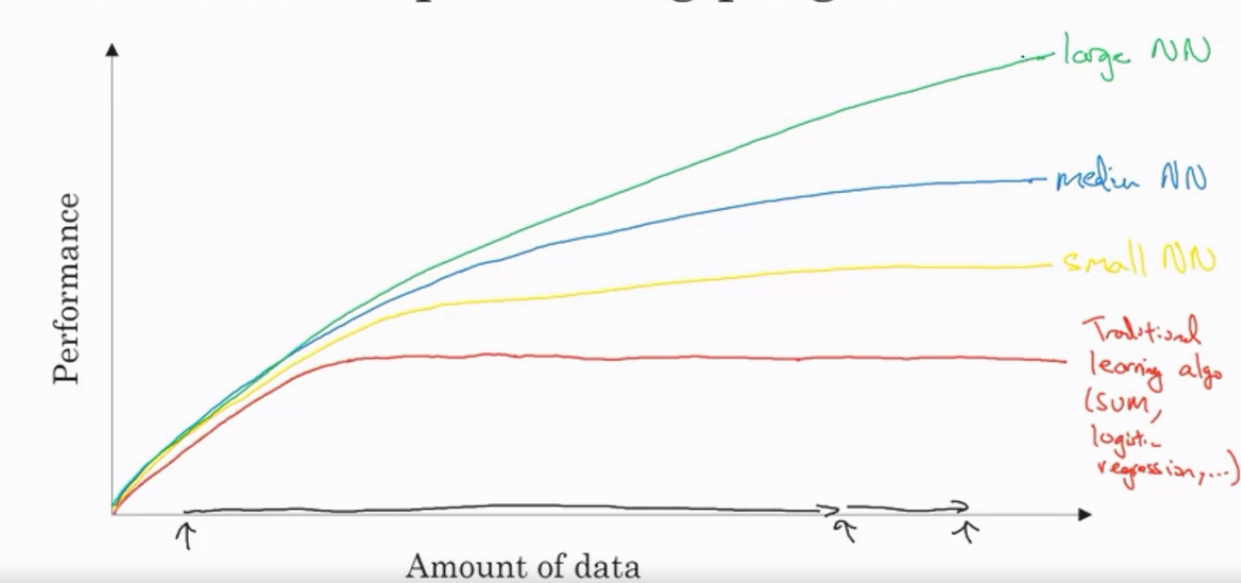
\includegraphics[scale=0.4]{Res/ml_algorithms_performance.png}
\caption{The performance of machine learning algorithms in respect to the data
we provide to them.}
\label{ml_algorithms_performance.png}
\end{figure}

We also see in the graph that when we don't have a large amount of data, NNs
all algorithms perform pretty much the same.

So in order to answer our question, we have to understand the evolution of three
things: \textit{data}, \textit{computation} and \textit{algorithms}.

Through the years, the amount of data available was inscreased a lot, so NNs can
take advantage from that. Also the computation power was inscreased with the use
of GPUs to make a large amount of computations. And finally new algorithms have
been developed to make NNs faster. That's the main reason why deep learning is
taking off.

\section{Notation}%
\label{sec:notation}

Before continuing, we need to define the notation we're going to use.

\begin{itemize}
    \item $(x,y)$ will denote a single training input;
    \item $m$ or $m_{\text{train}}$ denotes the number of training examples;
    \item $\xii[x]{i}$ denotes the $i$-th training input;
    \item $\xii[y]{i}$ denotes the $i$-th traning output;
    \item $n_x$ or $n$ denotes the number of dimensions $x$ has (or the number
        of features);
    \item $m_{\text{test}}$ denotes the number of testing examples;
    \item $X$ is the matrix of all traning examples. It's defined as:
        \[
        X = \begin{bmatrix}
            | & | &  & | \\
            \xii[x]{1} & \xii[x]{2} & \cdots & \xii[x]{m} \\
            | & | &  & | \\
        \end{bmatrix}
        \]
        $X$ is an $m\times n$ matrix;
    \item $Y$ is the matrix of all outputs. It's defined as:
        \[
        Y = \begin{bmatrix}
            \xii[y]{1} & \xii[y]{2} & \cdots & \xii[y]{m}
        \end{bmatrix}
        \]
        $Y$ is a $1\times m$ matrix.
\end{itemize}

\begin{obs}
In other courses we might see $X$ defined as the transpouse of the matrix we've
just defined. But it turns out that when using this definiting, it's much easier
to implement algorithms, so remember te definition we're going to use through out
the course.

The same thing for $Y$. We see that here $Y$ is the transpouse of that it's
tends to be in other courses.
\end{obs}

\section{Logistic Regression as a Neural Network}%
\label{par:logistic_regression_as_a_neural_network}

To end this introduction, we'll see the basics of neural network programming
using the simplest NN we can: a logistic regression.

So let's recall what's logistic regression and why it's useful. Logistic
Regression is used in binary classification, the kind of problem where we have
an input and want to predict between $0$ or $1$. An example could be an image
and we want to say it what's a cat ($1$) or not ($0$).

Basicly we want an algorhthm to estimate the probability of $y=1$ given $x$. In
math we write:
\[
    \hat{y}=P(y=1\cond x),\t\t x\in\R^{n}
\]

Logistic Regression estimates this quantity using the formula:

\[
    \hat{y}=\sigma(w^{T}x+b),
\]
where $w$ and $b$ are parameters to be discovered and $\sigma$ is the
\textbf{sigmoid function}:

\[
    \sigma(z) = \dfrac{1}{1+e^{-z}}
\]

\begin{figure}[h]
\centering
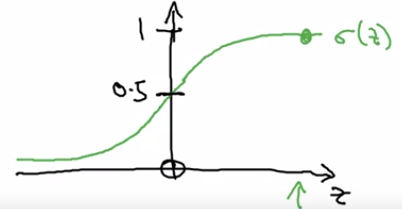
\includegraphics[scale=0.7]{Res/sigmoid.png}
\caption{A sigmoid graph.}
\label{sigmoid.png}
\end{figure}

It's also common to create a new input $x_0=1$ and use the $x$ vector as
$x\in\R^{n+1}$ and use the formula $\hat{y}=\sigma(\theta^{T}x)$, where

\[
\theta=\begin{bmatrix}
    \theta_0 \\ \theta_1 \\ \theta_2 \\ \vdots \\ \theta_n
\end{bmatrix}\t \theta_0=b\t w=\begin{bmatrix}
    \theta_1 \\ \theta_2 \\ \vdots \\ \theta_n
\end{bmatrix}
\]

To find the parameters $b$ and $w$, we need to define a \textbf{cost function},
which is a function that says how badly our algorithm is performing. This is a
function that we want to minimize and when we minimize, we find the best values
of $b$ and $w$.

The \textbf{cost} function is a function of all training examples, while a
\textbf{loss function} or \textbf{error function} is a function of a single
traning example that measures how well our algorithm is performing.

For logistic regression, we use the loss function:

\[
    \mathcal{L}(\hat{y},y)=-y \log\hat{y}-(1-y)\log(1-\hat{y})
\]

Notice that this is the same as:
\[
    \mathcal{L}(\hat{y},y)=\begin{cases}
        -\log(\hat{y}-1), &\text{ if } y=0\\
        -\log\hat{y}, &\text{ if } y=1\\
    \end{cases}
\]

That give us the cost function:
\[
    J(w,b)=\dfrac{1}{m}\spsum{i=1}{m}\mathcal{L}(\xii[\hat{y}]{i},\xii[y]{i})
\]

\subsection{Gradient Descent}%
\label{sub:gradient_descent}

We know have:
\begin{itemize}
    \item A way of predicting the classes $0$ or $1$ using the sigmoid function;
    \item A way of measuring the error of our predictions.
\end{itemize}

What we need now is a way of chaning our parameters $b$ and $w$ in order to
minimize the error. That's what the \textbf{gradient descent} algorithm does.

Let's first see a general graph of the cost function. In general, it looks like
figure \ref{Cost_function.png}

\begin{figure}[h]
\centering
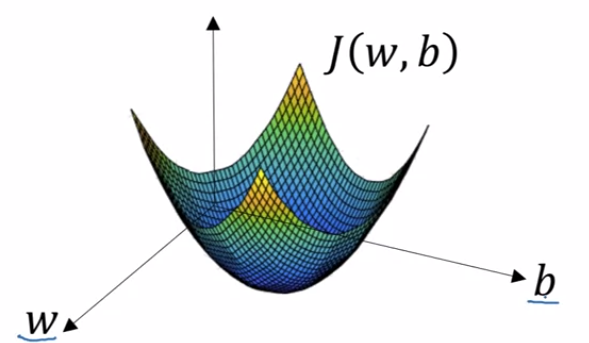
\includegraphics[scale=0.8]{Res/Cost_function.png}
\caption{A generic graph of the cost function.}
\label{Cost_function.png}
\end{figure}

We see that $J$ is what we call a \textbf{convex function}, which means that it
is a function that was only one \textbf{local minimum} (or local maxima). This
property is very important if we want to apply the gradient descent algorithm.

In Gradient Descent, we initialize $b$ and $w$ randomly and take steps into the
direction that leads us to the lowest possible value of $J$. In order to do
that, we calculate the \textbf{gradient} (the derivatives in each direction) of
the function $J$ and take a step in the opposite direction of the gradient.

\begin{prop}
The gradient gives us the direction of the maximum increase of the a function.
\end{prop}

\begin{algorithm}[Gradient Descent]
Repeat \{ \nl
\t $w:=w-\alpha\parderiv[w]{J(w,b)}$ \nl
\t $b:=b-\alpha\parderiv[b]{J(w,b)}$ \nl
\}
\end{algorithm}

In the algorithm, $\alpha$ is what we call the \textbf{learning rate}. It's how
large we should step in the direction of the maximum decrease. If we take big
steps, we can go much faster to the global minumum, but we might not be so
accurated. On the other hand, we be take small steps, we can find the global
minum accuratedly, but achieve it much slower.

Gradient Descent is a general optimization algorithm and can be applied to any
convex function. So now we need to understand how to use it with logistic
regression.

After calculating the derivatives, we'll have:

\begin{algorithm}[Gradient Descent for Logistic Regression]
Repeat \{ \nl
\t$J=0;~dw=0;~db=0$ \nl
\t For $i=1\cdots m$:\nl
\t\t $\xii[z]{i}=w^{T}\xii[x]{i}+b$\nl
\t\t $\xii[a]{i}=\sigma(\xii[z]{i})$\nl
\t\t $J+=
-\sbracket{\xii[y]{i}\log\xii[a]{i}+(1-\xii[y]{i})\log(1-\xii[a]{i})}$\nl
\t\t $d\xii[z]{i}=\xii[a]{i}-\xii[y]{i}$\nl
\t\t $dw += \xii[x]{i}d\xii[z]{i}$\nl
\t\t $db += d\xii[z]{i}$\nl
\t $J/=m$\nl
\t $dw/=m;~db/=m$\nl
\t $w:=w-\alpha dw$ \nl
\t $b:=b-\alpha db$ \nl
\}
\end{algorithm}

This version of the algorithm uses a for loop to compute $J$, $dw$ and $db$. But
when implementing the code into Python or other language, we always try to
\textbf{vectorize} the code to make it faster.

\begin{algorithm}[Gradient Descent for Logistic Regression Vectorized]
Repeat \{ \nl
\t $Z=w^{T}X+b$ \nl
\t $A=\sigma(Z)$ \nl
\t $dZ = A - Y$ \nl
\t $dw = \dfrac{1}{m}XdZ^{T}$ \nl
\t $db = \dfrac{1}{m}\spsum{}{}dZ$ \nl
\t $w:=w-\alpha dw$ \nl
\t $b:=b-\alpha db$ \nl
\}
\end{algorithm}

%%%%%%%%%%%%%%%%%%%%%%%%%%%%%%%%%%%%%%%%%%%%%%%%%%%%%%%%%%%%%%%%%%%%%%%%%%%%%%%%

\end{document}
